\documentclass[11pt,compress,t,notes=noshow, aspectratio=169, xcolor=table]{beamer}

\usepackage{../../style/lmu-lecture}
% Defines macros and environments
% This file is included in slides and exercises

% Rarely used fontstyle for R packages, used only in 
% - forests/slides-forests-benchmark.tex
% - exercises/single-exercises/methods_l_1.Rnw
% - slides/cart/attic/slides_extra_trees.Rnw
\newcommand{\pkg}[1]{{\fontseries{b}\selectfont #1}}

% Spacing helpers, used often (mostly in exercises for \dlz)
\newcommand{\lz}{\vspace{0.5cm}} % vertical space (used often in slides)
\newcommand{\dlz}{\vspace{1cm}}  % double vertical space (used often in exercises, never in slides)
\newcommand{\oneliner}[1] % Oneliner for important statements, used e.g. in iml, algods
{\begin{block}{}\begin{center}\begin{Large}#1\end{Large}\end{center}\end{block}}

% Don't know if this is used or needed, remove?
% textcolor that works in mathmode
% https://tex.stackexchange.com/a/261480
% Used e.g. in forests/slides-forests-bagging.tex
% [...] \textcolor{blue}{\tfrac{1}{M}\sum^M_{m} [...]
% \makeatletter
% \renewcommand*{\@textcolor}[3]{%
%   \protect\leavevmode
%   \begingroup
%     \color#1{#2}#3%
%   \endgroup
% }
% \makeatother


\title{Interpretable Machine Learning}
% \author{LMU}
%\institute{\href{https://compstat-lmu.github.io/lecture_iml/}{compstat-lmu.github.io/lecture\_iml}}
\date{}

\begin{document}

\newcommand{\titlefigure}{figure_man/me_movement}
\newcommand{\learninggoals}{
\item Why parameter-based interpretations are not always possible for parametric models
\item How marginal effects can be used in such cases
\item Drawbacks of marginal effects
\item Model-agnostic applicability}

\lecturechapter{Marginal Effects}
\lecture{Interpretable Machine Learning}

\begin{frame}{Interpretation of Simple Models}

\begin{itemize}
\itemsep1em
\item LM: Change in $x_1$ by $\Delta x_1$ results in change in $y$ by $\Delta y = \Delta x_1 \cdot \theta_1$
%interpretation  characterized by feature coefficients:
\begin{equation*}
y = \theta_0 + \theta_1 x_1 + \dots + \theta_p x_p + \dots + \epsilon
\end{equation*}
%\item A change in $x_1$ by $\Delta x_1$ results in a change in $y$ by $\Delta y = \Delta x_1 \cdot \theta_1$
\item Default interpretations correspond to $\Delta x_1 = 1$, i.e., $\Delta y = \theta$
\item All under "ceteris paribus", i.e., all remaining features are kept constant
\item For polynomial models with higher-order or interaction terms, interpretations via single coefficients are not possible anymore, e.g.:
%\begin{equation*}

\medskip

\centerline{$y = \theta_0 + \theta_{1} x_1^2 + \theta_{2} x_2^2 + \theta_{1, 2} x_1 \cdot x_2 + \epsilon$}

\medskip

%\label{eq:poly_model}
%\end{equation*}
\begin{itemize}
%
\item Marginal effect of feature $x_1$ varies across different values for feature $x_2$ (and vice versa)
\item Interaction depends on values of another feature
%\item If $x_1$ changes, $y$ is affected by $\theta_1$ and $\theta_{1,2}$ 
\end{itemize}
\end{itemize}
\end{frame}

% \begin{frame}{Interpretations of Polynomial Models}


% \begin{itemize}
% \itemsep1em
% \item If higher-order terms or interactions are present, parameter-based interpretations are not possible anymore:
% \begin{equation}
% y = \theta_0 + \theta_{1} x_1^2 + \theta_{2} x_2^2 + \theta_{1, 2} x_1, x_2 + \epsilon
% \label{eq:poly_model}
% \end{equation}
% \item The isolated main effects of both features vary across different values
% \item The interaction depends on values of the remaining feature
% \item The marginal effect allows us to determine a feature effect nonetheless.
% \end{itemize}

% \end{frame}

\begin{frame}{Marginal Effects}

\begin{itemize}
%\itemsep2em
\item
Derivative ME: Derivative of $f$ w.r.t. feature. Compute via numeric differentiation
$$dME_j(x) = \frac{\partial f(x)}{\partial x_j} \approx \frac{f(x + h) - f(x - h)}{2h}$$
\item Less known definition based on forward differences: Change in predicted outcome due to a change in feature value (e.g., increasing a feature $x_j$ by $h_j$) $\Rightarrow$ forward ME (fME):
\begin{equation*}
fME_j(x, h_j) = f(x_1, \dots, x_j + h_j, \dots, x_p) - f(x)
\end{equation*}
\item Example: For model equation $y = \theta_0 + \theta_{1} x_1^2 + \theta_{2} x_2^2 + \theta_{1, 2} x_1 \cdot x_2 + \epsilon$
\begin{itemize}
\item dME of $x_1$ is $dME_1(x) = 2\theta_1 x_1 +  \theta_{1, 2} x_2$
\item fME of $x_1$ with step size $h_1 = 1$ is
$fME_1(x, h_1) = 2\theta_1 h_1^2 +  \theta_{1, 2} x_2 h_1$
\end{itemize}
\end{itemize}
\end{frame}


%%%

\begin{frame}{Derivative versus Forward Difference}

%%%

\begin{columns}[T]
\begin{column}{0.6\textwidth}
\begin{itemize}
\itemsep1em
\item Derivative of non-linear prediction functions substantially differ at different points \\
$\Rightarrow$ dME is not suited
\item fME corresponds to a movement on prediction function, indicating changes in predicted outcome regardless of the function's shape\\
$\Rightarrow$ fME better suited for non-linear prediction functions
\item However, with both variants, we lose information about the prediction function along the finite difference
\end{itemize}
\end{column}
\begin{column}{0.4\textwidth}
 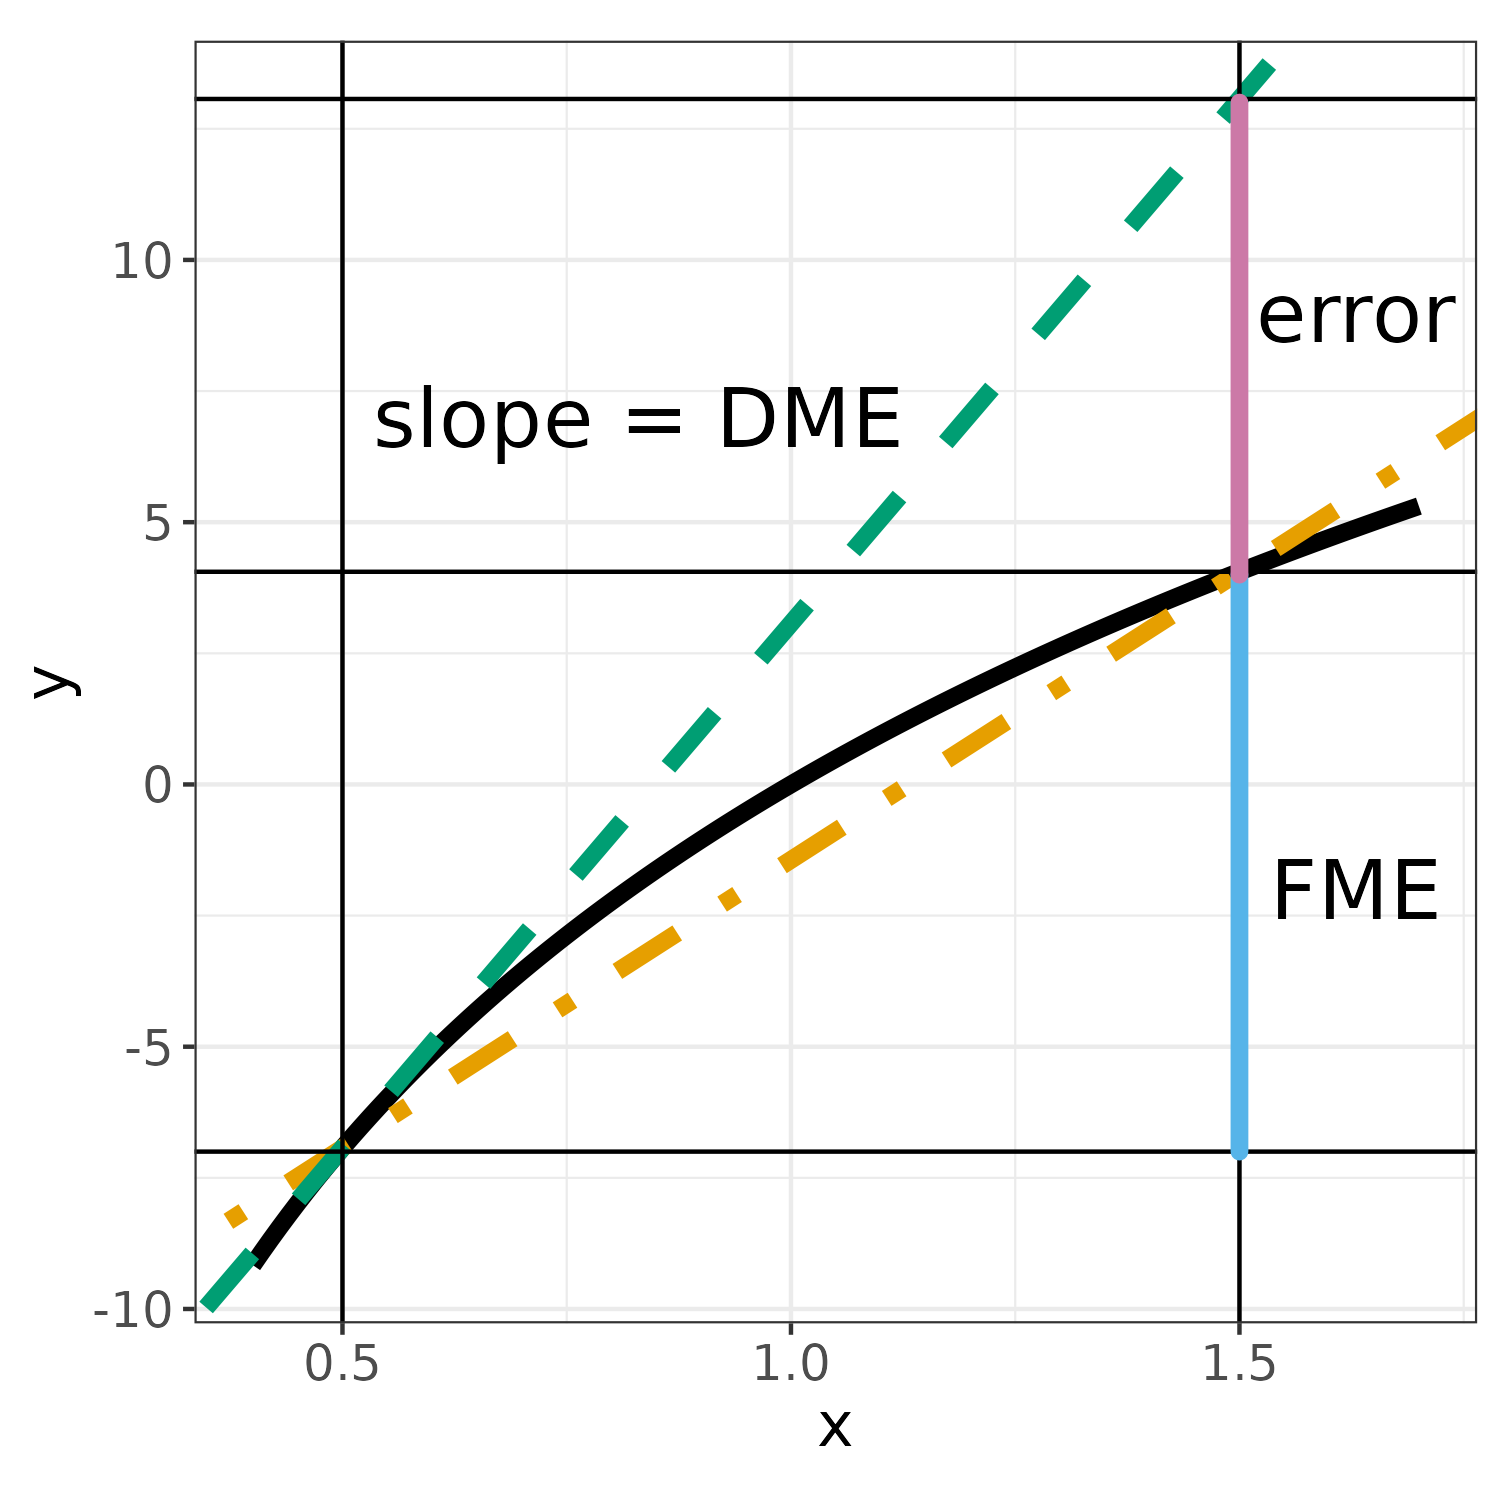
\includegraphics[width = \textwidth]{figure_man/derivative_me_error.png}
\end{column}
\end{columns}

\end{frame}

% \begin{frame}{Derivative versus Forward Difference}
% \begin{figure}
%   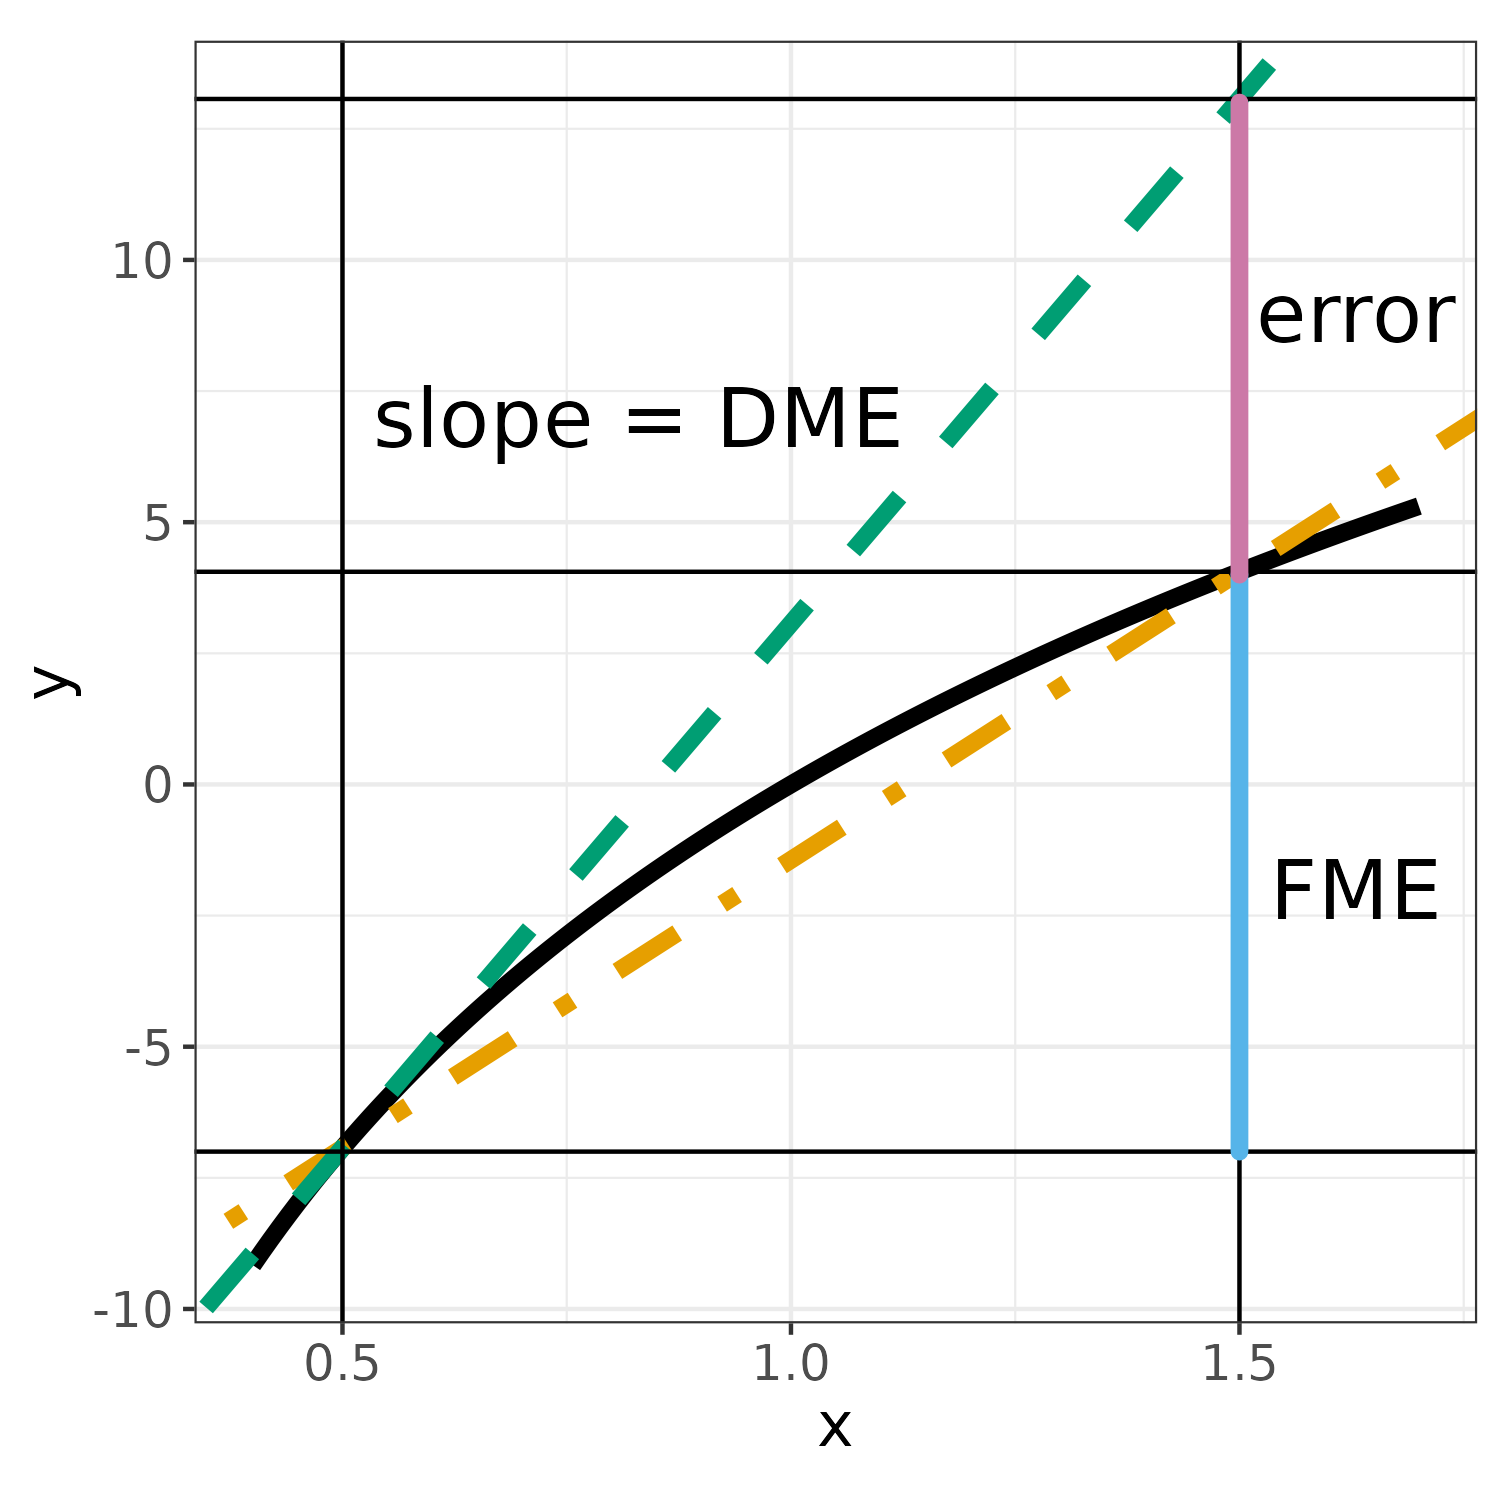
\includegraphics[width = 0.5\textwidth]{figure_man/derivative_me_error.png}
% \end{figure}
% \end{frame}

\begin{frame}{Additive Recovery}

\begin{itemize}
\itemsep1em
\item Both variants only recover terms within prediction function that depend on feature(s) of interest
\item Consider a prediction function $\widehat{f}(x) = ax_1 + bx_2$. It follows that:
\begin{align*}
dME_1(x) &= a \\
fME_1(x, h_1) &= ah_1
\end{align*}
\item MEs remove effects of other features that are linked additively, regardless of how many remaining features exist, and their effect structure
\end{itemize}

\end{frame}


\begin{frame}{Model-Agnostic Applicability}

\begin{itemize}
\itemsep1em
\item MEs were historically used to interpret GLMs, however, they can be used as model-agnostic interpretation tools for non-parametric models 
%\item As fMEs are better suited for non-linear prediction functions, they are better suited for interpreting ML models
\item fMEs correspond to an exploration of the prediction function and are better suited for non-linear prediction functions
\item With fMEs, we can also use multivariate changes in feature values to explore the prediction surface in various directions simultaneously
\item Note: Shape of the prediction function may vary considerably along the forward difference, i.e., an fME with half the step size may not result in half the fME
\end{itemize}

\end{frame}


% \begin{frame}{Model-Agnostic Applicability}

% \begin{itemize}
% \itemsep2em
% \item MEs are traditionally used to interpret parametric models such as GLMs. However, both dME and fME can be used as model-agnostic interpretation tools for non-parametric models. As the fME is better suited for non-linear prediction functions, it is the natural choice for black box ML models.
% \item The fME essentially correspond to an exploration of the prediction function. We can also use multivariate changes in feature values to explore the prediction surface in various directions simultaneously.
% \item One needs to keep in mind that the shape of the prediction function may vary considerably along the forward difference, i.e., an fME with half the step size may not result in half the fME.
% \end{itemize}

% \end{frame}





\endlecture
\end{document}
